% Options for packages loaded elsewhere
\PassOptionsToPackage{unicode}{hyperref}
\PassOptionsToPackage{hyphens}{url}
%
\documentclass[
  12pt,
]{article}
\usepackage{amsmath,amssymb}
\usepackage{iftex}
\ifPDFTeX
  \usepackage[T1]{fontenc}
  \usepackage[utf8]{inputenc}
  \usepackage{textcomp} % provide euro and other symbols
\else % if luatex or xetex
  \usepackage{unicode-math} % this also loads fontspec
  \defaultfontfeatures{Scale=MatchLowercase}
  \defaultfontfeatures[\rmfamily]{Ligatures=TeX,Scale=1}
\fi
\usepackage{lmodern}
\ifPDFTeX\else
  % xetex/luatex font selection
\fi
% Use upquote if available, for straight quotes in verbatim environments
\IfFileExists{upquote.sty}{\usepackage{upquote}}{}
\IfFileExists{microtype.sty}{% use microtype if available
  \usepackage[]{microtype}
  \UseMicrotypeSet[protrusion]{basicmath} % disable protrusion for tt fonts
}{}
\makeatletter
\@ifundefined{KOMAClassName}{% if non-KOMA class
  \IfFileExists{parskip.sty}{%
    \usepackage{parskip}
  }{% else
    \setlength{\parindent}{0pt}
    \setlength{\parskip}{6pt plus 2pt minus 1pt}}
}{% if KOMA class
  \KOMAoptions{parskip=half}}
\makeatother
\usepackage{xcolor}
\usepackage[margin=1in]{geometry}
\usepackage{graphicx}
\makeatletter
\def\maxwidth{\ifdim\Gin@nat@width>\linewidth\linewidth\else\Gin@nat@width\fi}
\def\maxheight{\ifdim\Gin@nat@height>\textheight\textheight\else\Gin@nat@height\fi}
\makeatother
% Scale images if necessary, so that they will not overflow the page
% margins by default, and it is still possible to overwrite the defaults
% using explicit options in \includegraphics[width, height, ...]{}
\setkeys{Gin}{width=\maxwidth,height=\maxheight,keepaspectratio}
% Set default figure placement to htbp
\makeatletter
\def\fps@figure{htbp}
\makeatother
\setlength{\emergencystretch}{3em} % prevent overfull lines
\providecommand{\tightlist}{%
  \setlength{\itemsep}{0pt}\setlength{\parskip}{0pt}}
\setcounter{secnumdepth}{5}
\usepackage{setspace,lscape} \usepackage{amsmath} \usepackage{array} \usepackage{caption,subcaption} \usepackage{longtable} \usepackage{booktabs} \usepackage{enumitem} \usepackage{standalone} \renewcommand{\arraystretch}{1.5} \captionsetup[table]{skip=5pt} \setstretch{1.5}
\ifLuaTeX
  \usepackage{selnolig}  % disable illegal ligatures
\fi
\usepackage[]{natbib}
\bibliographystyle{apalike}
\IfFileExists{bookmark.sty}{\usepackage{bookmark}}{\usepackage{hyperref}}
\IfFileExists{xurl.sty}{\usepackage{xurl}}{} % add URL line breaks if available
\urlstyle{same}
\hypersetup{
  pdftitle={Results of Experiment 2},
  pdfauthor={Zark Zijian Wang},
  hidelinks,
  pdfcreator={LaTeX via pandoc}}

\title{Results of Experiment 2}
\author{Zark Zijian Wang}
\date{February 10, 2024}

\begin{document}
\maketitle

\hypertarget{sample}{%
\section{Sample}\label{sample}}

In this experiment, each subject was required to complete a same survey.
The survey contains 4 choice questions for consistency check, 14
fill-in-the-blank questions as the main task, and one additional choice
question for measuring impatience.

In each fill-in-the-blank question, participants will face two reward
sequences - Option A and Option B. Option A offers two rewards at two
specific times: one today and another after a certain delay (e.g.
``receive £185 today and £60 in 6 months''). Option B offers an unknown
amount today and no amount after the same delay. Participants have to
identify which level of this unknown amount would make them value the
two options equally, and fill in the blank with their answer. Figure
\ref{fig:fill-blank-screen} presents an example question. We term their
answer as the ``indifference point'' between the two options. Throughout
the survey, the back-end amount in Option A is fixed at £60. We set up
seven levels for the front-end amount (£25, £105, £185, £265, £345,
£425, £505), and two levels for the delay (6 months and 12 months.
Overall, there are 14 fill-in-the-blank questions, presented in a random
order.

\begin{figure}
  \vspace{16pt}
  \centering
  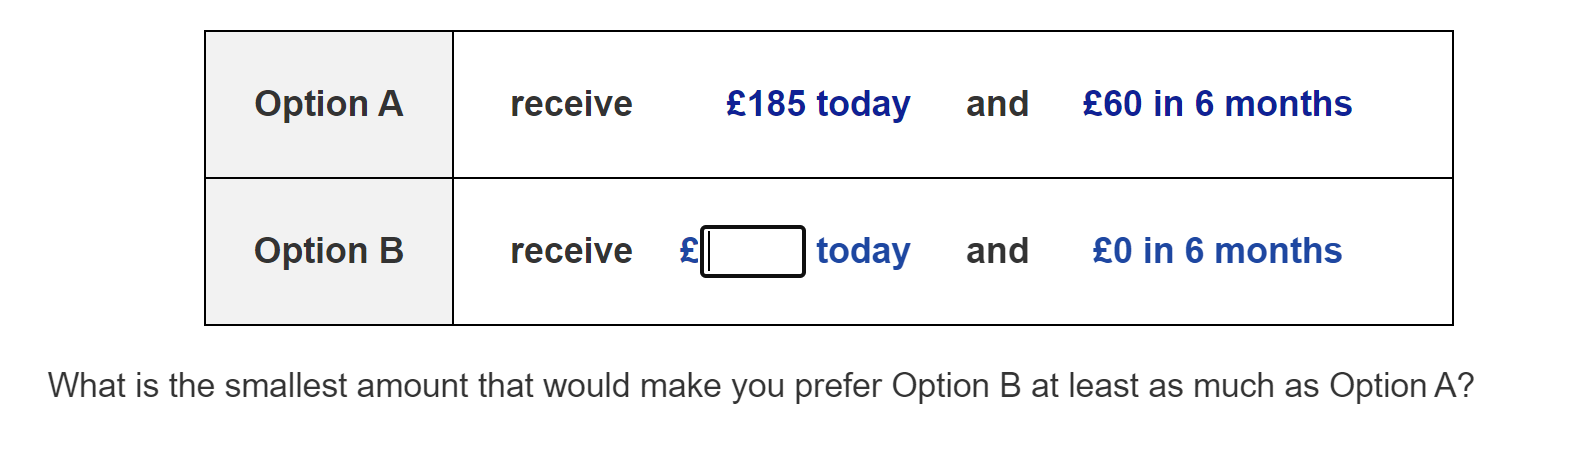
\includegraphics[width=0.96\textwidth]{figures/screenshot.png}
  \caption{Screenshot of an fill-in-the-blank question}
  \label{fig:fill-blank-screen}
\end{figure}

Before participants start doing the main task, there are four
consistency check questions. Each consistency check question contains
two options: one is the same as Option A in a subsequent
fill-in-the-blank question; the other is framed in the way as Option B,
offering a specific amount today and no amount in the certain delay. In
the latter option, the amount offered today is either the same as that
of the former option, or above the total money in the former option.
Participants are required to choose the option they prefer. We exclude
the participants whose choices are incompatible with their answers in
the correponding fill-in-the-blank questions. For example, a participant
may face a choice between ``receive £185 today and £60 in 6 months'' and
``receive £300 today and £0 in 6 months''. If she choose the latter
option, then when she meets the former option in a subsequent
fill-in-the-blank question, she should fill in an amount smaller than
£300. Finally, at the end of the survey, we add one additional question
to measure the participants' impatience. The question is the same as the
``Preference for Earlier vs Later Income'' (PELI) task in
\citet{burro2022patience}.

Two hundred subjects (female: 50\%) were recruited via Prolific, of
which 197 subjects completed the survey\footnote{When a question was
  loaded multiple times during the survey completion process, the survey
  will be automatically ended and submitted, in order to prevent
  duplicate responses. This situation occurred with three participants.
  We thus abort their answers.}. The median age for those who completed
the survey is 38, the median completion time is 4.8 minutes. The minimum
completion time is 1.83 minutes. We offer £1.2 for each participant.
There were 157 subjects having passed the consistency check. Given that
each subject completed 14 fill-in-the-blank questions, we construct a
sample of 2,198 observations.

\hypertarget{heterogeneity-in-responses}{%
\section{Heterogeneity in Responses}\label{heterogeneity-in-responses}}

\hypertarget{regression-results}{%
\section{Regression Results}\label{regression-results}}


\documentclass[12pt]{article}


\begin{document}
\begin{table}
    \caption{Regression Results}
    \vspace*{12pt}
    \centering

      \begin{tabular}{lllllll}
\hline
 & (1) Pool & (2) Pool & (3) FE & (4) FE & (5) RLM & (6) RLM \\
\hline
$Y_1\cdot1\{T=T_L\}$ & -0.005$^{**}$ &  & -0.005$^{*}$ &  & -0.005$^{***}$ &  \\
 & (0.002) &  & (0.002) &  & (0.001) &  \\
$Y_1\cdot1\{T=T_H\}$ & -0.006$^{***}$ &  & -0.005$^{**}$ &  & -0.006$^{***}$ &  \\
 & (0.002) &  & (0.002) &  & (0.001) &  \\
$Y_1\cdot1\{T=T_L\}\times$CL1 &  & 0.022$^{***}$ &  & 0.002 &  & 0.0 \\
 &  & (0.004) &  & (0.002) &  & (0.001) \\
$Y_1\cdot1\{T=T_H\}\times$CL1 &  & 0.023$^{***}$ &  & 0.003 &  & -0.0 \\
 &  & (0.004) &  & (0.002) &  & (0.001) \\
$Y_1\cdot1\{T=T_L\}\times$CL2 &  & -0.06$^{***}$ &  & -0.019$^{***}$ &  & -0.017$^{***}$ \\
 &  & (0.005) &  & (0.004) &  & (0.002) \\
$Y_1\cdot1\{T=T_H\}\times$CL2 &  & -0.062$^{***}$ &  & -0.021$^{***}$ &  & -0.022$^{***}$ \\
 &  & (0.005) &  & (0.004) &  & (0.002) \\
PELI & -0.239 & -0.645 & 9.187$^{***}$ & 7.215$^{***}$ & 2.181$^{***}$ & 2.206$^{***}$ \\
 & (3.95) & (2.638) & (0.015) & (0.364) & (0.319) & (0.31) \\
Constant & 53.742$^{***}$ & 54.037$^{***}$ & 46.434$^{***}$ & 47.965$^{***}$ & 52.158$^{***}$ & 52.385$^{***}$ \\
 & (3.619) & (2.684) & (0.485) & (0.432) & (0.361) & (0.351) \\\hline

observations & 2186 & 2186 & 2186 & 2186 & 2198 & 2198 \\
adj-$R^2$ & 0.0 & 0.334 & 0.648 & 0.654 &  &  \\
Muller-Welsh &  &  &  &  & 128.457 & 122.183 \\
\hline
\end{tabular}
% INSERT reg_combined

    \vspace*{4pt}
    \centering
    \begin{minipage}{1.0\textwidth}
    {\par\footnotesize Note: * $p<0.05$, ** $p<0.01$, *** $p<0.001$. Standard errors are reported in the parentheses. Model (1)-(2) are pooled OLS models, model (3)-(4) are fixed-effect OLS models, model (5)-(6) are fixed-effect robust linear regressions (RLM). For OLS, standard errors are clustered at the subject level, and p-values are calculated using t-tests. For RLM, each model is estimated using Huber's M-estimator (the threshold for loss function is set at 1.345) and the scale estimator is Huber's proposal 2 estimator. Each p-value for RLM is calculated based on a normal distribution with i.i.d. assumption. A smaller Muller-Welsh score indicates the model has a greater ability to both parsimoniously fit the data and predict new independent obeservations. $Y_1$ and $T$ denote the front-end amount and the sequence length in Option A. $T_L$ and $T_H$ are 6 months and 12 months, respectively. Clustering results are obtained through k-means method.}
    \end{minipage}
    \label{tab:seq_value_reg}
\end{table}

\end{document}



\hypertarget{discussion}{%
\section{Discussion}\label{discussion}}

\renewcommand\refname{Reference}
  \bibliography{experiment-2-ref.bib}

\end{document}
